\chapter*{КОНТРОЛЬНЫЕ ВОПРОСЫ}
\addcontentsline{toc}{chapter}{КОНТРОЛЬНЫЕ ВОПРОСЫ}

\begin{enumerate}
	\item Что называется дешифратором?
	
	Дешифратор -- комбинационный узел с $n$ входами и $N$ выходами, преобразующий каждый набор двоичных сигналов в активный сигнал на выходе, соответствующий этому набору.
	
	\item Какой дешифратор называется полным (неполным)?
	
	Дешифратор, имеющий $2n$ выходов, называется полным, при меньшем числе выходов -- неполным.
	
	\item Определите закон функционирования дешифратора аналитически и таблично.

	\begin{figure}[h]
		\centering
		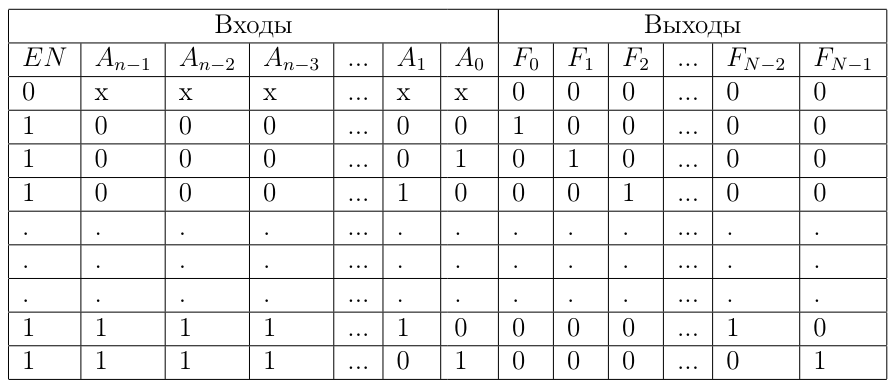
\includegraphics[width=\linewidth]{img/question3-table}
	\end{figure}

	Аналитически описать дешифратор можно совокупностью логических функций в СДНФ:
	
	\pagebreak

	\begin{figure}[ht]
		\centering
		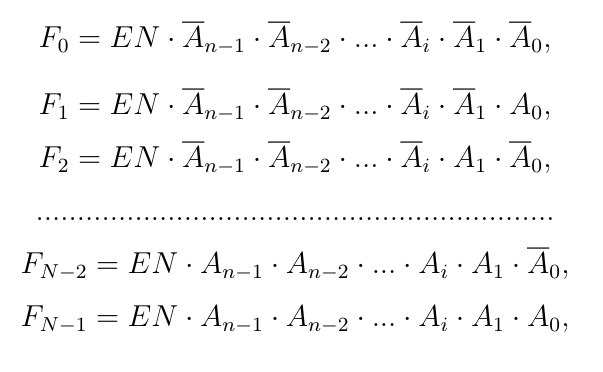
\includegraphics[width=0.6\linewidth]{img/question3-eq}
	\end{figure}

	\item{Поясните основные способы построения дешифраторов.}

	Линейный дешифратор строится в соответствии с системой, представленной в предыдущем вопросе, и представляет собой $2n$ конъюнкторов или логических элементов ИЛИ-НЕ
	с $n$-входами каждый при отсутствии стробирования и с $n + 1$ входами -- при его наличии.
	Пирамидальный дешифратор строится на основе последовательной (каскадной) реализации выходных функций. На первом этапе реализуются конъюнкции двух переменных.
	На втором -- все конъюнкции трех переменных путем логического умножения каждой ранее полученной конъюнкции двух переменных на переменную. Таким образом, на каждом
	следующем этапе получают вдвое больше конъюнкции, чем на предыдущем. Пирамидальные дешифраторы независимо от числа их входов строятся на основе только двухвходовых конъюнкторов.
	
	\item{Что называется гонками и как устраняются ложные сигналы, вызванные гонками?}
	
	Вследствие переходных процессов и временных задержек сигналов в цепях логических элементов могут возникнуть так называемые гонки, приводящие к появлению ложных сигналов на выходах схемы. Основным средством, позволяющим исключить гонки, является стробирование (выделение из информационного сигнала той части, которая свободна от искажений, вызываемых гонками). Стробирующий сигнал на этом входе не должен
	быть активным во время переходных процессов в дешифраторе.
	
	\item{Каковы способы наращивания дешифраторов по количеству входов и выходов и как они реализуются схемотехнически?}
	
	Пусть для построения сложного дешифратора $DC$ $n - N$ используются простые дешифраторы $DC$ $n_1 - N_1$, причем $n_1 << n$, следовательно $N_1 << N$.
	
	Число каскадов равно $K = \frac{n}{n_1}$: если $K \in \mathbb{Z}$, то во всех каскадах используются полные дешифраторы $DC$ $n_1 - N_1$. Если $K$ -- правильная или смешанная дробь, то во входном каскаде используется неполный дешифратор $DC$ $n_1 - N_1$.
	
	Количество простых дешифраторов $DC$ $n_1-N_1$ в выходном каскаде равно $\frac{N}{N1}$, в предвыходном - $\frac{N}{N_1^2}$, в предпредвыходном - $\frac{N}{N_1^3}$ и т.д.; во входном каскаде -- $\frac{N}{N_1^k}$. Если $\frac{N}{N_1^k}$ -- правильная дробь, то это означает, что во входном каскаде используется неполный простой дешифратор.
	
	В выходном каскаде дешифрируются $n_1$ младших разрядов адреса сложного
	дешифратора, в предвыходном – следующие $n_1$ младших разрядов адреса сложного дешифратора и т.д. Во входном каскаде дешифрируется полная или неполная группа старших разрядов адреса. Поэтому $n_1$ младших разрядов адреса сложного дешифратора подаются параллельно на адресные входы всех дешифраторов выходного каскада, следующие $n_1$ младших разрядов адреса -- на адресные входы всех дешифраторов предвыходного каскада и т.д.; группа старших разрядов адреса подается на адресные входы дешифратора.
	
	Выходы дешифраторов предвыходного каскада соединяются с входами разрешения
	простых дешифраторов выходного каскада, выходы дешифраторов
	предпредвыходного каскада -- с входами разрешения простых дешифраторов
	предвыходного каскада и т.д.
	
\end{enumerate}
